\section{Antenna Design 1 -- Minimized Monopole}
\label{sec:techsol1_monopole_5mm}
The minimized monopole design and the tuning schematic can be seen on Figure \ref{fig:ant1techschem_6pf}. The design is still based on the first folded monopole design, but is made smaller and simpler without any folding.

\begin{figure}[htbp]
    \begin{subfigure}[b]{0.49\linewidth}
        \centering
        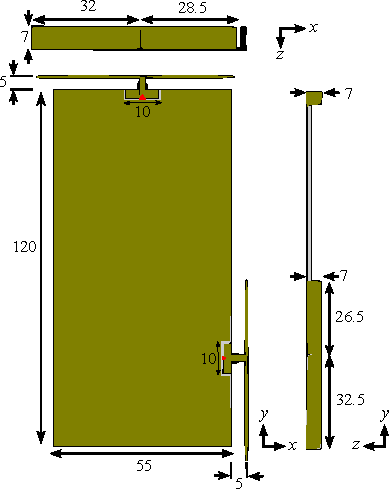
\includegraphics{img/tech_sol/monopole/5mm/3d_drawing/3d_drawing}
        \caption{Technical drawing.}
        \label{fig:ant1technical_6pf}
    \end{subfigure}
    \hfill
    \begin{subfigure}[b]{0.49\linewidth}
        \centering
        \includegraphics{img/tech_sol/schematic_tuning_1}\\[1cm]
\footnotesize
        \begin{tabular}{|l|l|l|l|}
            \hline
            & $C_1$ & $L_1$ & $C_2$ \\
            \hline
            Top antenna & \SI{3.02}{pF} & \SI{7.99}{nH} & $[0.3,2.9]\,$pF\\
            Side antenna & \SI{1.81}{pF} & \SI{5.27}{nH} & $[0.3,2.9]\,$pF\\
            \hline
        \end{tabular}
        \caption{Tuning/matching circuit.}
        \label{fig:ant1_tuning}
    \end{subfigure}
    \caption{Technical drawing and tuning circuit for the antenna.  The matching circuit is applied for both the top and the side antenna.}
    \label{fig:ant1techschem_6pf}
\end{figure}

The ground clearence S11 and efficiency simulation can be seen on Figure \ref{fig:eff_s11_mono_sim_5mm}.
The simulation sweep is done from \SI{10}{mm} to \SI{3}{mm} ground clearence in \SI{1}{mm} steps and only for the top antenna. Each ground clearence simulation is matched and tuned to get the highest bandwidth possible.

From the S11 results it is clear that the bandwidth decreases as the ground clearence decreases. The most noticeable results is at \SI{5}{mm} clearence as the bandwidth from this point does not increase significantly when increasing the ground clearence. However decreasing the ground clearence further to \SI{4}{mm} and \SI{3}{mm} the bandwidth drops significantly. Based on these results is was chosen to minimize the antenna design to a ground clearence of \SI{5}{mm}.

The effieicncy ground clearence comparison shows some similar results. In the high band it's clear that decresing the ground clearence will also decrease the bandwidth. However the high band results seems hard to compare, as the different simulations is matched at different frequencies to gain the highest bandwidth. The comparison is more noticeable in the low band, where it is clear, that the lower the clearence the lower the efficiency. Generally the effieicncy does not drop that much when decreasing the ground clearence. It should also be possible to increase the efficiency and compensated for the drop with tuning.  

\begin{figure}[htbp]
   \begin{subfigure}[b]{0.49\linewidth}
        \centering
        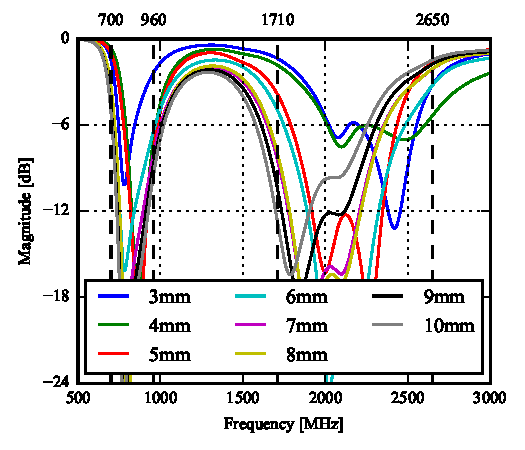
\includegraphics{img/tech_sol/monopole/5mm/s11_5mm}
        \caption{S11 parameter for the top antenna, when sweeping the ground clearence.}
        \label{fig:s11_mono_sim_5mm}
    \end{subfigure}
    \hfill
    \begin{subfigure}[b]{0.49\linewidth}
        \centering
        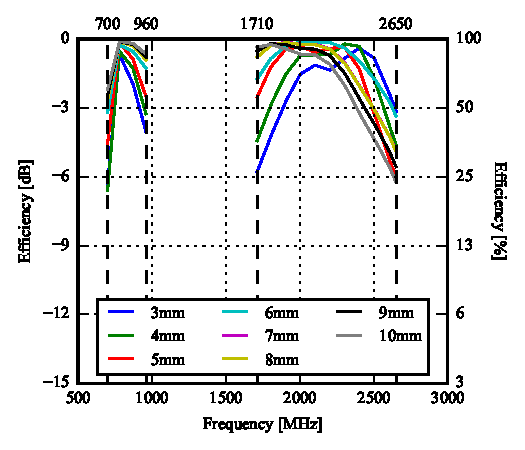
\includegraphics{img/tech_sol/monopole/5mm/eff_5mm}
        \caption{Efficiency for the top antenna, when sweeping the ground clearence.}
        \label{fig:eff_mono_sim_5mm}
    \end{subfigure}
    \caption{S11 and efficiency for the top antenna, when sweeping the ground clearence from \SI{3}{mm} to \SI{10}{mm}}
    \label{fig:eff_s11_mono_sim_5mm}
\end{figure}

Furthermore a sweep on the antenna height was also carried out from \SI{7}{mm} to \SI{4}{mm}. The results are not included as the top antenna was unable to cover the high band at anything lower than \SI{7}{mm} in height.


The simulated S-parameter for both the top and the side antenna can be seen on Figure \ref{fig:ant1_6pf_sparam}. The bandwidth results can be seen in Table \ref{tab:bw_sol1_6pf}. Both antennas fulfill the requirement for the low band and in the high band only the top antenna experiences some problems. The top antenna lacks \SI{76}{MHz} of bandwidth in the high band. The lack of \SI{76}{MHz} band width is acceptable as it covers close to the \SI{720}{MHz} requirement.

The tuned S-parameters for both antennas can be seen in Figure \ref{fig:sparam_mono_6pf_free_space}. From the results it is seen that both antennas covers the entire low band. In the high band only the top antenna experiences some minor problems of \SI{-1}{dB} and \SI{-3}{dB} loss in the band limits. The isolation loss have improved a bit comparing with the results from the first design, but is still significant in the lower band.     

The tuned efficiency for both antennas can be seen in Figure \ref{fig:eff_sol1_6pf_free}. From the results it is seen that both antennas are capable of covering the high band with an efficiency of \SI{50}{\percent} or higher. In the low band a lot of tuning is needed to achieve a efficiency around \SI{50}{\percent}. Generally the efficiency drops as the capacity increases as expected.  

% S-parameters at C1 and C3 = 0.6pf
\begin{figure}[htbp]
    \centering
    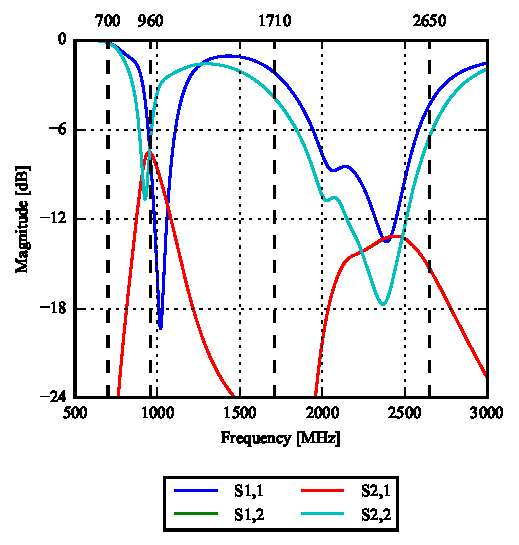
\includegraphics{img/tech_sol/monopole/5mm/6pf_sparams}
    \caption{S-parameters with $C_2=\SI{0.3}{pF}$ for both antennas.}
    \label{fig:ant1_6pf_sparam}
\end{figure}

%bandwidth table
\begin{table}
  \centering
  \begin{tabular}{|l|l|r|r|r|}
    \hline
    Antenna & Band & Start [MHz] & Stop [MHz] & Bandwidth [MHz] \\
    \hline
    Top     & Low  & 882         & 963       & 81 \\
    Side    & Low  & 943         & 1108        & 165 \\
    \hline
    Top     & High & 1945        & 2589       & 644 \\
    Side    & High & 1842        & 2671       & 849 \\
    \hline
  \end{tabular}
  \caption{Maximum bandwidth obtained in the low and high band for the top and the side antenna, respectively.}
  \label{tab:bw_sol1_6pf}
\end{table}

% Sweeping S-parameters
\begin{figure}[htbp]
   \begin{subfigure}[b]{0.49\linewidth}
        \centering
        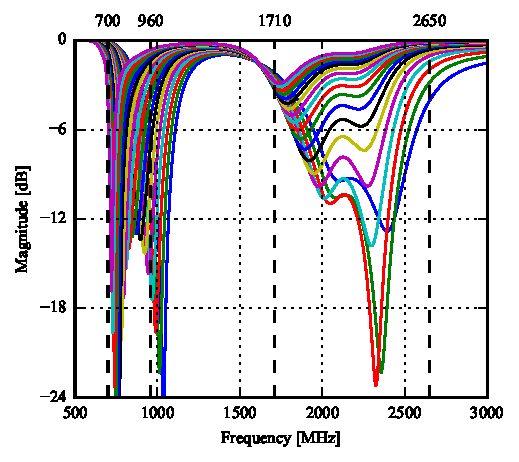
\includegraphics{img/tech_sol/monopole/5mm/6pf_s11}
        \caption{$S_{11}$, sweeping $C_1$ and fixing $C_2$.}
    \end{subfigure}
    \hfill
    \begin{subfigure}[b]{0.49\linewidth}
        \centering
        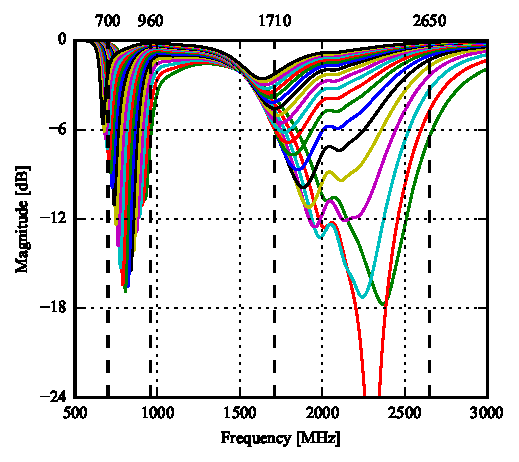
\includegraphics{img/tech_sol/monopole/5mm/6pf_s22}
        \caption{$S_{22}$, sweeping $C_2$ and fixing $C_1$.}
    \end{subfigure}
~
    \begin{subfigure}[b]{0.49\linewidth}
        \centering
        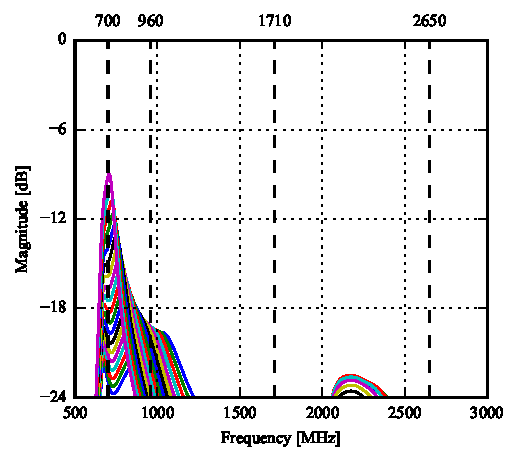
\includegraphics{img/tech_sol/monopole/5mm/6pf_s11_s21}
        \caption{$S_{21}$, sweeping $C_1$ and fixing $C_2$.}
    \end{subfigure}
    \hfill
    \begin{subfigure}[b]{0.49\linewidth}
        \centering
        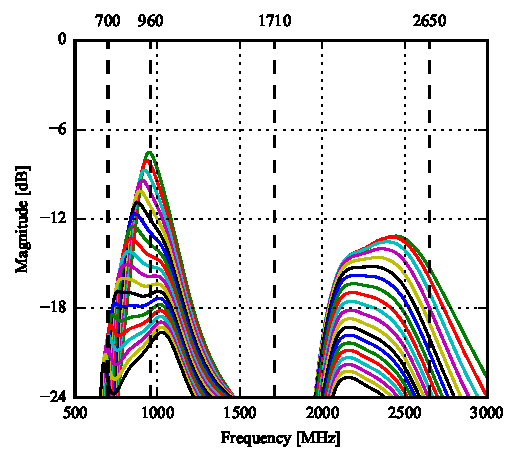
\includegraphics{img/tech_sol/monopole/5mm/6pf_s22_s21}
        \caption{$S_{21}$, sweeping $C_2$ and fixing $C_1$.}
    \end{subfigure}
    \caption{S-parameter sweep in free space for tuning the shunt capacitor of each antenna, $C_1$ and $C_2$ for port 1 and 2, respectively. Port 1 is the top antenna and port 2 is the side antenna.}
    \label{fig:sparam_mono_6pf_free_space}
\end{figure}

% Sweeping Efficiency
\begin{figure}[htbp]
    \centering
    \begin{subfigure}{0.49\linewidth}
        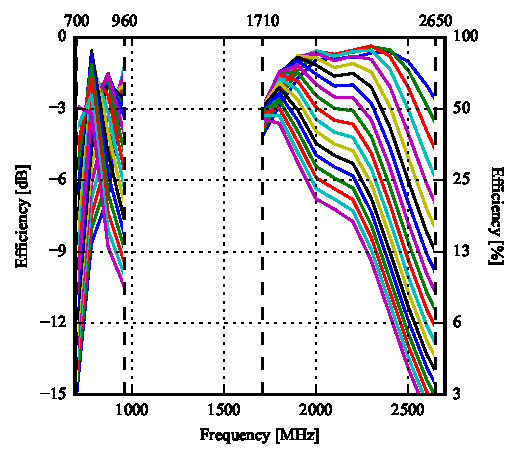
\includegraphics{img/tech_sol/monopole/5mm/6pf_eff_ac1}
        \caption{Sweeping $C_1$ and fixing $C_2$.}
    \end{subfigure}
    \hfill
    \begin{subfigure}{0.49\linewidth}
        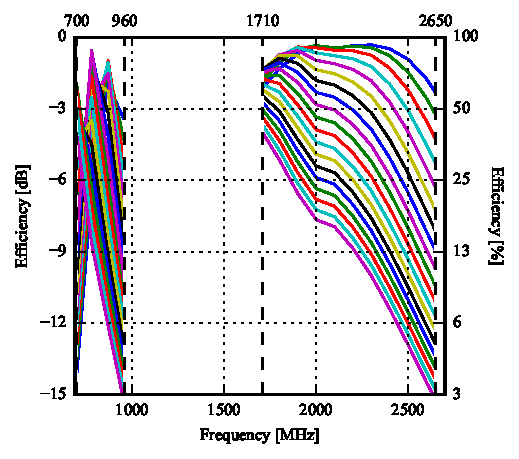
\includegraphics{img/tech_sol/monopole/5mm/6pf_eff_ac2}
        \caption{Sweeping $C_2$ and fixing $C_1$.}
    \end{subfigure}
    \caption{Efficiency for each antenna when sweeping the tunable capacitors. Here, $C_1$ and $C_2$ are the tuning capacitor for the top and side antenna, respectively.}
    \label{fig:eff_sol1_6pf_free}
\end{figure}


